\paragraph{IUE04 Visualizar Practicantes} \hspace{1cm}\\
\label{pant:IUE04}

\textbf{\textcolor[rgb]{0, 0, 0.545098}{Objetivo}}\\
Esta pantalla permite al Entrenador visualizar a cada uno de los Practicantes registrados en la herramienta. Además de permitirle realizar diferentes acciones para cada uno de ellos.\\

\textbf{\textcolor[rgb]{0, 0, 0.545098}{Diseño}}\\
La figura \ref{fig:IUE04} muestra al Entrenador una lista con los identificadores (imagen y nombre) de los Practicantes registrados. Los Practicantes se visualizan en una lista horizontal ordenados alfabéticamente.\\

En la parte inferior se encuentra el botón de Regresar, el cual corresponde a mostrar la pantalla previa a ésta.\\

Cada una de las imágenes de los identificadores tiene una función de botón, la cual muestra un menú de opciones.\\

\begin{figure}[H]
	\centering
		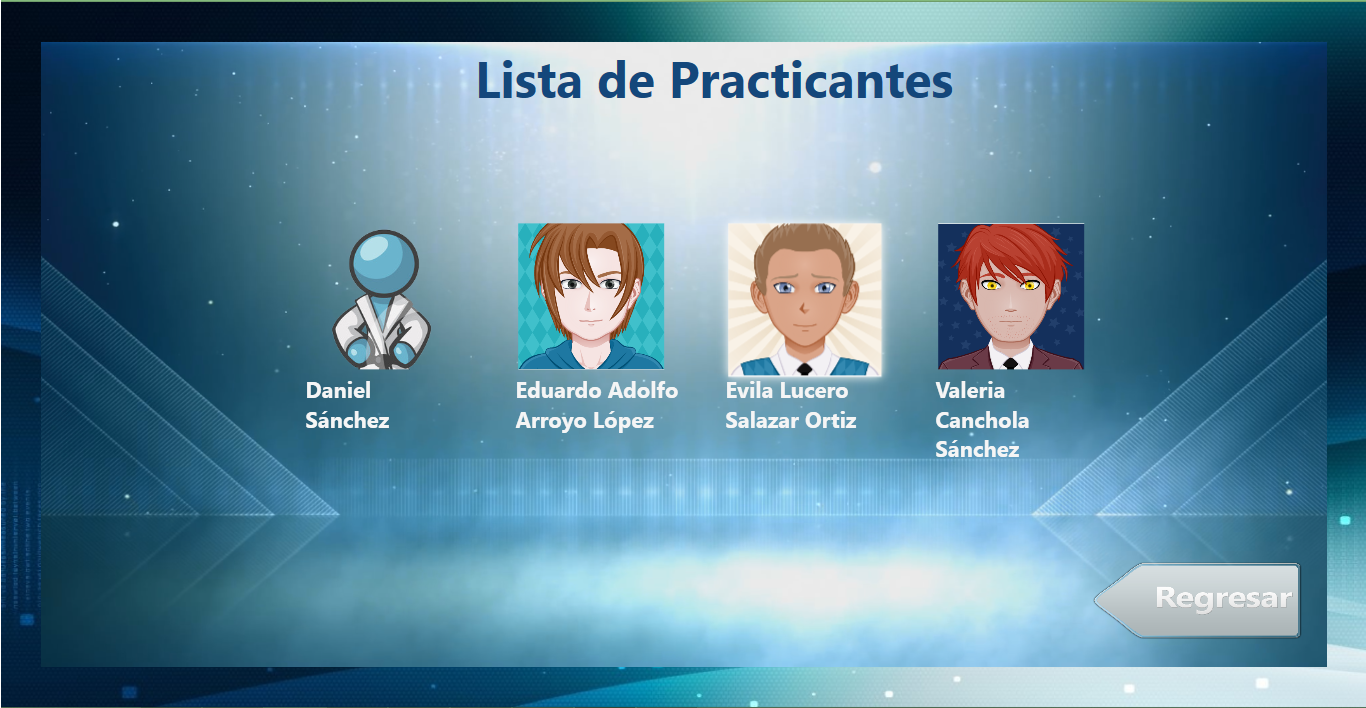
\includegraphics[scale=0.5]{./Figuras/Pantallas/IUE04Visualizar_Practicantes}
	\caption{IUE04 Lista de Practicantes}
	\label{fig:IUE04}
\end{figure}

\textbf{\textcolor[rgb]{0, 0, 0.545098}{Comandos}}
\begin{itemize}
	\item \textbf{\textcolor[rgb]{0, 0, 0.545098}{Regresar:}} Regresa al menú \nameref{menu:ME02}.
	\item \textbf{\textcolor[rgb]{0, 0, 0.545098}{Imagen (Identificador):}} Muestra al Entrenador el menú \nameref{menu:ME04}.	
\end{itemize}
\vspace{1em}

\textbf{\textcolor[rgb]{0, 0, 0.545098}{Mensajes}}\\

\nameref{msj:MSG24}: Se muestra en el menú principal \nameref{menu:ME02} cuando cuando debido a un error de conexión no se muestren los elementos de forma correcta.\\

\clearpage